\subsection{Vorticity and polarization}

An interesting open question for relativistic fluids is to what extent the 
  spin degrees of freedom thermalize locally and to what extend spin 
  polarization results as a consequence of the fluid motion. 
Intuitively, one might expect that spin aligns locally with the rotational 
  motion of the fluid as measured by vorticity, corresponding to the curl 
  of the fluid velocity.

The relativistic generalization of the non-relativistic fluid vorticity is 
  not unambiguous, however. 
The vorticity of a fluid in local equilibrium is characterized by the so-called 
  thermal vorticity tensor, corresponding to $\omega_{\mu\nu} = \frac{1}{2} 
  (\nabla_\nu \beta_\mu - \nabla_\mu \beta_\nu)$ where $\beta_\mu=u_\mu / T$ 
  is the ratio of fluid velocity to temperature~\cite{Becattini:2013fla}. 
This thermal vorticity includes contributions from global rotational motion, 
  local fluid acceleration, and temperature gradients. 
It has been argued that this thermal vorticity should lead to local 
  spin polarization. 
If this holds at chemical freeze-out, one should be able to find traces of the 
  thermal vorticity in the spin polarization of particles and resonances, 
  such as $\Lambda$ ($\overline{\Lambda}$) particles.

Spin polarization is in this picture closely tied to angular momentum of the 
  expanding fireball. 
For non-central events, an angular momentum of the produced matter can be 
  generated that is perpendicular to the event plane. 
Via the spin-vorticity coupling mechanism, this leads to a global polarization 
  in the transverse plane aligning with the global angular momentum (also known 
  as the ``transverse polarization''). 
This global transverse polarization has recently been found in the measurement 
  of $\Lambda$ spin polarization at RHIC~\cite{STAR:2017ckg}. 
For this global effect following global angular momentum, one expects a 
  decreasing magnitude with increasing collision energy and the effect is 
  expected to be relatively small at LHC energies. 

\begin{figure*}[!htb]
\begin{center}
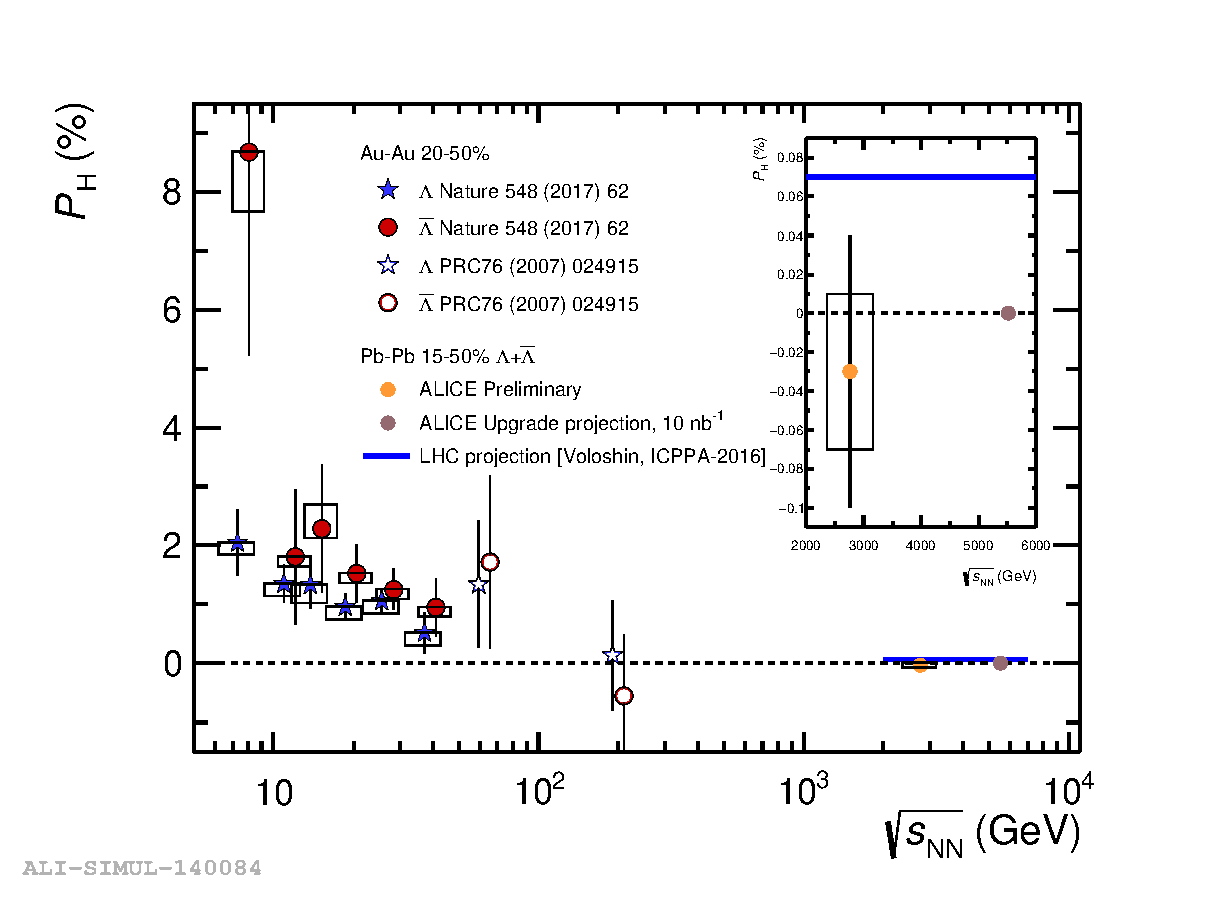
\includegraphics[width=0.8\textwidth]{\main/flow/figs/alice_projection_lambda}
\caption{
ALICE projections for the Global hyperon polarization in \pbpb\ 
  collisions at $\snn=2.76$~TeV for an integrated luminosity of 
  10~nb$^{-1}$ (blush symbol), together with the present measurements (orange symbol) 
  compared to analogous measurements at various collision energies from the STAR 
  collaboration~\cite{STAR:2017ckg, Abelev:2007zk} (blue and red symbols). 
The blue line indicates the prediction for the maximum value at the 
  LHC~\cite{Voloshin:ICPPA2}. 
The inlay plot shows a zoomed in version of the plot around the ALICE 
  measurement and Run~3 and 4 projection, together with the prediction 
  for the maximum value at the LHC.
The points for $\overline{\Lambda}$ are slightly shifted along the horizontal 
  axis for visibility.  
Error bars (open boxes) represent the statistical (systematic) uncertainties.}
\label{fig:alice_lambda}
\end{center}
\end{figure*}

Figure~\ref{fig:alice_lambda} shows the energy dependence of the global 
  transverse polarization of $\Lambda$ and $\overline{\Lambda}$ for
  semi-central heavy ion collisions. 
The RHIC results show the decrease of polarization with increasing \snn. 
%However, $\Lambda$ and $\overline{\Lambda}$ demonstrate finite global 
%  polarizations even at the highest RHIC energy of $\snn=200$~GeV~\cite{PRC-98-014910-2018}. 
The preliminary ALICE data point at $\snn=2.76$~TeV is consistent with zero
  within 1--$\sigma$ statistical/systematic uncertainties.
However it is also consistent with the predicted maximum value (blue line)
  within $\sim$2--$\sigma$ statistical/systematic uncertainties.
Thus unable to rule out both the null as well as non-zero signal cases.
But the ALICE upgrade projection at twice large collision energy,
  (made for the zero signal case) shows that the polarization in Run~3 
  and 4 can be measured with very high precision. 
Therefore the study of global polarization of $\Lambda$ and $\overline{\Lambda}$ 
  within HL--LHC project allows the unambiguous conclusion with regard of the 
  values of this physics quantity in the TeV-energy domain. 

In addition to the transverse polarization, an azimuthal-dependent, 
  longitudinal polarization (in the direction of the beam pipe) has 
  also been predicted. 
This is mainly a consequence of an azimuthal dependence of local acceleration 
  and temperature gradient (e.g., the elliptic flow), which could lead to an 
  elliptic modulation of longitudinal spin polarization in 
  non-central collisions. 
Unlike the global transverse polarization, this longitudinal polarization 
  effect has a much weaker dependence on collision energy from RHIC to 
  the LHC~\cite{Karpenko:2017dui}, mainly because the anisotropy flow has a 
  weak collision energy dependence. 
With increased data sample and upgraded detectors covering a wider rapidity 
  range in the HL--LHC era, there would be exciting opportunities to 
  investigate polarization effects of $\Lambda$ and other particles in great 
  detail at the LHC and to map out the dependence on azimuthal angle, 
  rapidity, transverse momentum etc.

%\begin{itemize}
%\item
%The estimation for the LHC energy $\snn=2.76$ TeV indicate the strength 
%of Abelian magnetic field is $eB \sim 1.0$ GeV$^{2}$ very shortly after 
%collisions and it decreases down to the $eB \sim 200$ MeV$^{2}$ for time 
%$\tau \sim 0.1$ fm/$c$ without taken into account the electroconductivity 
%of the quark-gluon matter \cite{AHEP-2014-193039-2014,JPCS-668-012129-2016,JPCS-675-022021-2016}. 
%Therefore one can expect $|\Delta P|=0.61eB/m_{p}T \sim (4.3 \pm 0.7) \times 10^{-4}$ 
%for the temperature of the quark-gluon plasma $T=(304 \pm 51)$ MeV \cite{NPA-904-905-573c-2013}. 
%Here $m_{p}$ is the proton mass, $\Delta P \equiv P_{\Lambda}-P_{\overline{\Lambda}}$ 
%is the difference in polarization of primary $\Lambda$ and $\overline{\Lambda}$ \cite{PRC-95-054902-2017}. 
%This estimation for $|\Delta P|$ is some smaller than that at RHIC energies 
%due to hotter medium at the LHC. But it should be noted the electroconductivity 
%will lead to noticeably weaker time dependence of the $eB$ \cite{AHEP-2013-490495-2013} 
%and the conductivity may compensate the growth of $T$ and provides the increase of 
%the $|\Delta P|$. Moreover the pass from RHIC to the LHC energy leads to the significant 
%growth of the peak value for $eB$. Thus for HE--LHC the magnitude of $\Delta P$ is 
%expected similar or even larger than at RHIC energies. Furthermore the higher energy 
%of the HE--LHC project provides the novel opportunity for study of polarization of 
%heavier hyperons (for instance, $\Sigma$) in hot environment.
%\end{itemize}


